\documentclass{article} % For LaTeX2e
\usepackage{nips13submit_e,times}
\usepackage[utf8]{inputenc}
\usepackage{hyperref}
\usepackage{graphicx}
\usepackage{url}
%\documentstyle[nips13submit_09,times,art10]{article} % For LaTeX 2.09

\title{Speech Generation with Recurrent Neural Networks}
\author{
Kyle Kastner\\
Département d’Informatique et de Recherche Opérationnelle\\
Université de Montréal, 2920 Chemin de la Tour, suite 2194,\\
Montréal (QC), H3T 1J4, Canada\\
\texttt{kastnerkyle@gmail.com} \\
}

% The \author macro works with any number of authors. There are two commands
% used to separate the names and addresses of multiple authors: \And and \AND.
%
% Using \And between authors leaves it to \LaTeX{} to determine where to break
% the lines. Using \AND forces a linebreak at that point. So, if \LaTeX{}
% puts 3 of 4 authors names on the first line, and the last on the second
% line, try using \AND instead of \And before the third author name.

\newcommand{\fix}{\marginpar{FIX}}
\newcommand{\new}{\marginpar{NEW}}

\nipsfinalcopy % Uncomment for camera-ready version

\begin{document}


\maketitle

\begin{abstract}
There are a wide variety of input 
representations and models used in speech
synthesis, with many research contributions from computer science, electrical
engineering, and statistics. One of the most promising models for capturing the
complex dynamics of speech is the recurrent neural network,
which holds state of the art results for the TIMIT speech recognition
task as well as many other complex time series problems. This paper will
discuss the particular concerns of applying recurrent neural networks to
perform speech generation, including datasets,
input representation, and modeling with recurrent neural networks.
\end{abstract}

\section{Outline}
The subsections below will
give a small introduction to recurrent neural networks and related topics
to be covered, with full coverage
reserved for the relevant section of the paper [1][2].

\subsection{Datasets}
Several datasets were used to evaluate this pipeline: speech data from the
TIMIT dataset, and speech data from the LibriSpeech dataset [3][4].

\subsection{Input Representations}
One of the most important parts of any machine learning pipeline is the
representation of the input. For speech synthesis, three different
representations are discussed: Linear Predictive Coding (LPC), sine wave
analysis, and raw input [5][6]. 

\subsection{Recurrent Neural Network Architectures}
Recurrent neural networks, like feedforward networks, have a staggering
number of possible configurations and hyperparameters. This work will focus on the
specific set of hyperparamters used for sequence generation,
as well as the unique difficulties in training such an architecture.

\section{Datasets}
Finding suitable datasets is one of the most difficult (though unheralded) 
problems in machine learning. Good speech datasets are particularly difficult
to find, since most corpora of labeled speech come from 
large corporations or have privacy concerns due to the nature of collection.
These datasets often hold identifying information from a large number of
people and are very expensive to label, store, secure, and curate.
\par
In this paper, the following qualifiers were used to select the datasets.
\begin{itemize}
    \item The data is well organized, with logical folder structure and naming conventions.
    \item The data is well documented, with README files or research reports detailing the collection environment.
    \item Examples are diverse, and span the range of conditions expected in "real world" usage. 
    \item The default resolution of examples is very high quality, and as close to "unprocessed" as possible.
\end{itemize}

Until very recently
with the release of the LibriSpeech dataset, most speech research
focused on the semi-public TIMIT dataset, with results on larger private
datasets which often change from publication to publication. In this research,
two primary datasets were used: the open and free LibriSpeech dataset, and
the open but non-free TIMIT dataset.
\subsection{TIMIT}
The TIMIT dataset is one of the most widely cited sets in speech processing research.
Though fairly small by recent standards, the TIMIT dataset features readings from 630 different speakers, with 10 different recordings from each speaker. The raw audio is stored as 16-bit, 16000 Hz wav files. It also features time-aligned orthographic, phonetic, and word labels for
each of the examples in the dataset. The labels and utterances have been hand verified by a number of researchers, and are considered to be the standard as far as audio and label granularity are concerned. The major downside to the TIMIT dataset is that it is non-free,
requiring a fairly substantial license fee to use. This can be prohibitive
for experimental research, or exploration by researchers whose primary focus
is not speech.
\subsection{LibriSpeech}
LibriSpeech is a new dataset published by researchers at
John Hopkins University. It is much larger than TIMIT, with approximately
1000 hours of recorded speech, including sentence level alignment and associated
text. The audio is formatted as 16-bit, 16000 Hz arff files, and is very
similar to TIMIT. It is free to use under the Creative Commons 4.0 license.
The primary drawback to using LibriSpeech is the granularity of labels and
tags, as sentence level alignment may not be sufficient for many speech
recognition tasks. For the purposes of unconditioned speech generation
this is not a problem.

\section{Input Representations}
How the data is formatted before being processed by the recurrent neural
network is crucial. Subtle differences in input representation from things
like mean centering, variance normalization, or removing correlation 
through transformations can be the difference between success and failure. For
the task of speech generation, there were three primary techniques
considered: "raw" input (mean centered and normalized as floating point from 0-1),
sinusoidal modeling, and Linear Predictive Coding (LPC).
\par
To understand how each of these methods transforms the input, it is first
necessary to understand a bit about the particulars of recorded speech. While
deep understanding of speech is a field of study to itself, there are a few
crucial details which make speech unique when compared to music
or other types of audio signals, and many of the input 
transformations used will exploit these details in some way.
\par
The building blocks of speech sounds are called phonemes - these are tiny
"sub-words" that are combined to make different words. Depending on which
phoneme is spoken, a segment of speech (sometimes called a frame) is considered
to be "voiced" or "unvoiced". The primary difference between these two
categories is that voiced speech has a very rich harmonic structure,
and is fairly straight forward to model. This includes sounds such as
"ooo" and "aaah". Unvoiced speech, on the other hand, includes silence,
growls, and explosive phonemes like "puh", "tuh", and "chk". These sounds
are typically more difficult to model, due to both the rapid onset of the
sounds and the brief duration relative to the voiced component. 

\subsection{Raw Input}
Raw input is a bit of a misnomer, as even in the "raw" case there are still
several things that must be done. Since the files are originally stored
as signed 16-bit values, the first step is to divide every sample by 2\^15.
This normalizes the input as floating point values in the (-1, 1) range, which
is normally small enough to avoid numerical problems. The other important
preprocessing step is to break the continuous speech into a number of
overlapping frames. The length and amount of overlap in the frame sizes can
vary, but a typical rule of thumb is 50\% overlap with frame sizes
capturing somewhere between 4 and 40 milliseconds of sound.
\par
For 16000 Hz,
this points to a frame size between 64 samples and 640 samples, with between
32 and 320 sample overlap. These numbers are chosen due to the dynamics of
speech, as each phoneme lasts (on average) about 10 milliseconds. Overlap is
crucial to providing context for the frame and relating it to what has been
seen, but there is a computational tradeoff as more overlap means
a larger computational overhead will be spent on redundant information.
Unfortunately, the network was unable to learn a useful representation of the
data for frame sizes greater than 5 or 10 samples. This makes learning very
difficult, due to the length of the hidden layers in time for the recurrent
network. Luckily, there are a few other preprocessing steps that can be taken
in order to find simpler representations for speech which may work well.

\subsection{Sinusoidal Modeling}
The Discrete Fourier Transform (and the temporal version, known as the STFT)
has a long history in the realm of speech
processing [7]. By taking the primary signal and breaking it down into a set of
sinusoids at different frequencies, we usually find the signal to be sparse in
frequency space. The transform has 
additional nice properties such as being orthogonal and linear. However, for
speech generation, a full Fourier basis is still very difficult to model, but it
is possible to reduce this set down to a few frequencies which contribute
most to making things sound
"speech-like". By estimating just 4 frequencies and their respective
gain coefficients it is possible to get a rough approximation of speech,
which should be easier to model than either the original time series or the
full Fourier transformed version. It also amounts a fairly large compression,
as the reduction from a frame size to 8 coefficients is quite large for any
reasonable frame size.

\subsubsection{Linear Predictive Coding}
Linear Predictive Coding (LPC) is a classic approach for robust
encoding and decoding of speech signals. It was originally designed for
use in low-bandwidth communications, but has also become the
standard for reconstruction quality due to Atal’s follow up work in perceptual
audio coding. It is also the one of the compression techniques specified in
the GSM phone standard. 
\par
The physical model used for LPC comes from observing that the human vocal
system is similar to a long pipe (the vocal tract) excited by a buzzer (the
tongue), with intermediate clicks and hisses (interactions of the tongue,
teeth, and lips). To create an approximate model in this way, a long speech
signal is broken into a series of overlapping frames. Each frame is modeled by
a linear component (an FIR filter), gain, and a residual which is not modeled
by the linear filter. This coded representation of the speech can then be
compressed and transmitted, or simply transmitted directly. 
\par
There are two primary modes for using decoding LPC: pure synthesis,
and residual driven synthesis. Pure synthesis does not use the residual
component during reconstruction. Instead, it uses an additional estimation of
whether the particular frame of speech was voiced, or unvoiced. It needs
estimation of the fundamental frequency of the frame. These are related to
the actual phoneme spoken, and many methods exist to make these measurements.
A signal (Gaussian random noise in the case of unvoiced, a pulse train at the
fundamental frequency for voiced) is then run through the filter given by the
LPC coefficients. In theory, the pulse wave is supposed to approximate
the glottal pulse created by the movement of the vocal tract, but the
approximation is quite crude and results in very “robotic” speech.
\par
The second mode of decoding LPC is residual driven synthesis. In this case,
the residual excitation is used to drive the filter given by the LPC
coefficients. In the case where all of the residual is kept, the
reconstruction is nearly perfect. By compressing this residual, we have the
ability to trade reconstruction quality for feature
dimensionality reduction. We strongly prefer the residual driven synthesis
mode, as this will give the most realistic reconstruction
and we are not particularly concerned with the ”bandwidth” cost of generating
a few extra features.

\section{Recurrent Architectures}
Recurrent neural networks are approximators for arbitrary dynamic systems.
This makes this type of architecture ideal for modeling data with rich
structure in both time and frequency, such as music or speech. The downside
to the raw power of recurrent neural networks is that training can be quite
difficult, and just like feedforward neural networks the hyperparamers
used for learning rate, learning rule, initialization, activation function, and
size of network have a massive impact on the performance for any specific
problem. The additional difficulty of using recurrent neural networks for
generation is that there needs to be an element of randomness. The default output of an RNN 
is deterministic based on the input, but we can still "seed" the
input and use the subsequent generations as input in a feedback loop to
generate different outputs.
\par
There are also more advanced methods of making the
RNN into a generative model, such as having the RNN learn
to predict the mean and variance parameters for a mixture of Gaussians,
rather than directly learning the output sequence. We have used this mixture of
Gaussians structure in all these experiments, in the
hopes of generating better and more unique samples. The downside to this
technique is increased variability in the output generation, especially if
the learned Gaussians have a broad covariance. This
will be discussed further in the results section.
\par
For the recurrent model, the same architecture is used for each
representation, only varying the input size and the output size for each
different dataset. It is key to remember that the output layer is a mixture of
Gaussians, which is then sampled to get data, rather than a direct mapping to
data space as is done in other recurrent architectures.
\begin{table}[ht]
\caption{Recurrent Network Hyperparameters} % title of Table
\centering % used for centering table
\begin{tabular}{p{4cm} c} % centered columns (4 columns)
\hline\hline %inserts double horizontal lines
Number of Hidden Layers & 3 \\% inserting body of the table
Activation & LSTM \\
Hidden Size & 300 \\
Output Gaussians & 20 \\
Learning Scheme & RMSProp \\
Learning Rate & 0.0001 \\
RMSProp Decay & 0.95 \\
RMSProp Momentum & .9 \\ 
Gradient Clipping & True \\
\hline %inserts single line
\end{tabular}
\label{table:hyperparams} % is used to refer this table in the text
\end{table}

\section{Results}

\begin{figure}[h!]
    \centering
    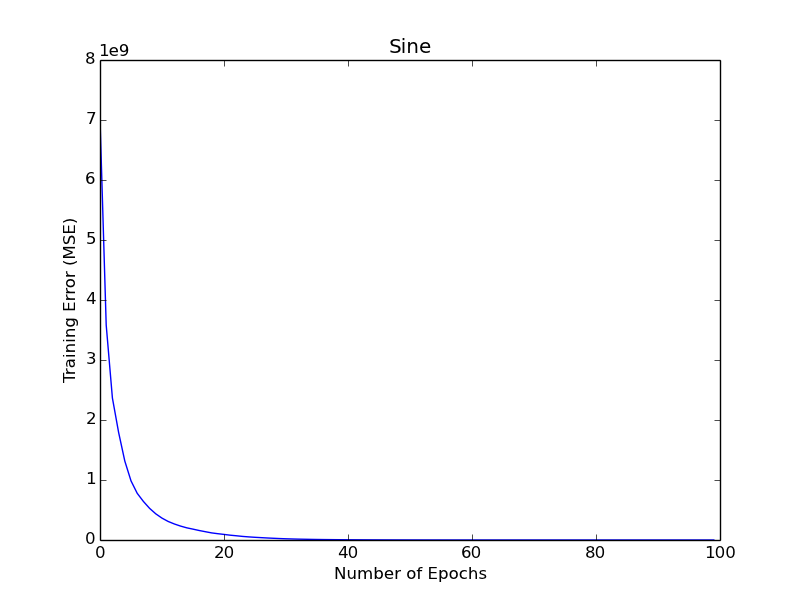
\includegraphics[width=0.6\textwidth,height=0.5\textwidth]{sine_error.png}
    \caption{Training on sinusoidal representation}
    \label{fig:sine_error}
\end{figure}

\begin{figure}[h!]
    \centering
    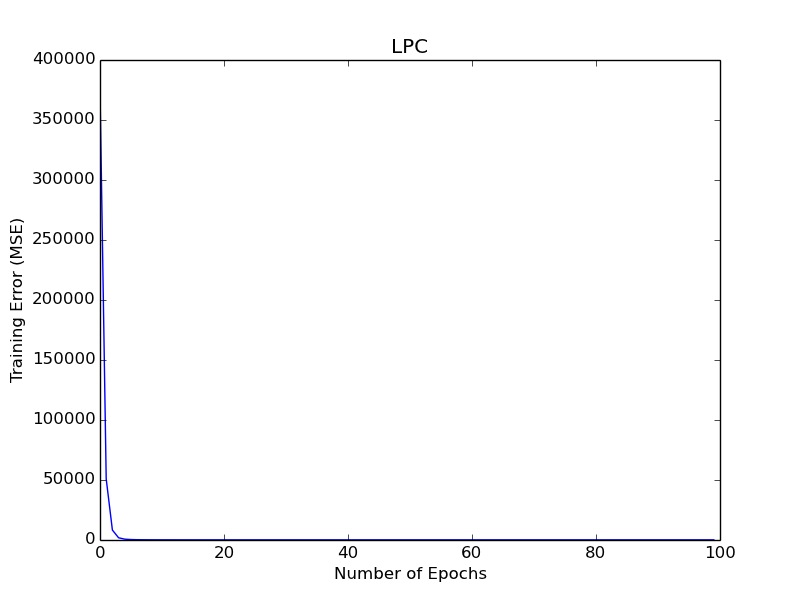
\includegraphics[width=0.6\textwidth,height=0.5\textwidth]{lpc_error.png}
    \caption{Training on LPC representation}
    \label{fig:lpc_error}
\end{figure}

\begin{figure}[h!]
    \centering
    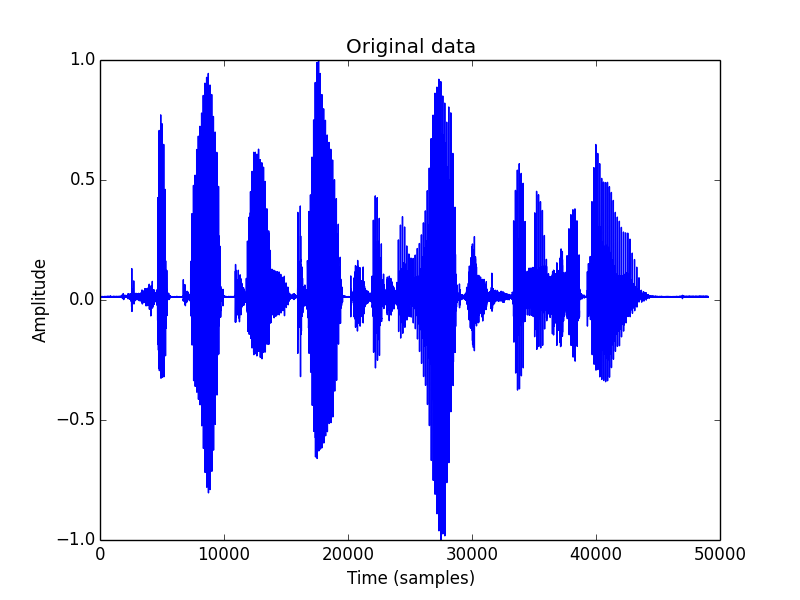
\includegraphics[width=0.6\textwidth,height=0.5\textwidth]{original_sample.png}
    \caption{Time domain sample of original speech}
    \label{fig:original_sample}
\end{figure}

\begin{figure}[h!]
    \centering
    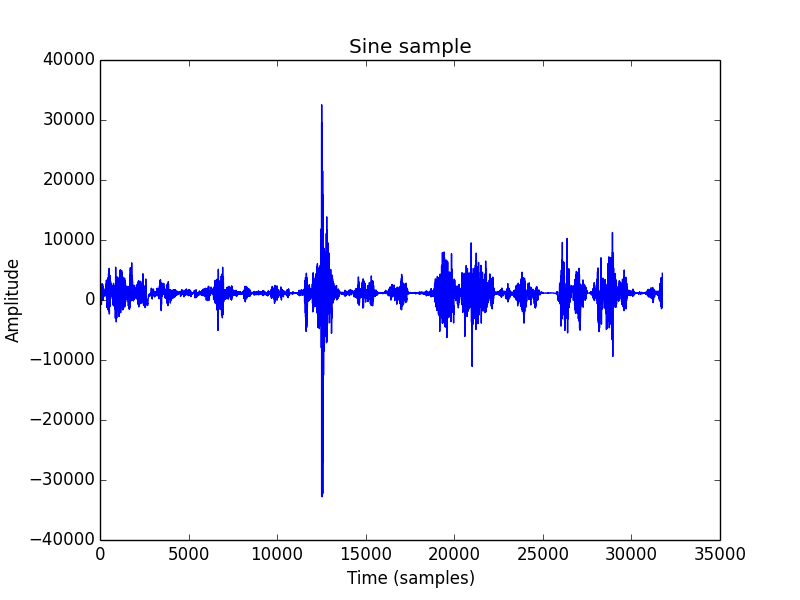
\includegraphics[width=0.6\textwidth,height=0.5\textwidth]{sine_sample.png}
    \caption{Time domain sample from sinusoidal model}
    \label{fig:sine_sample}
\end{figure}

\begin{figure}[h!]
    \centering
    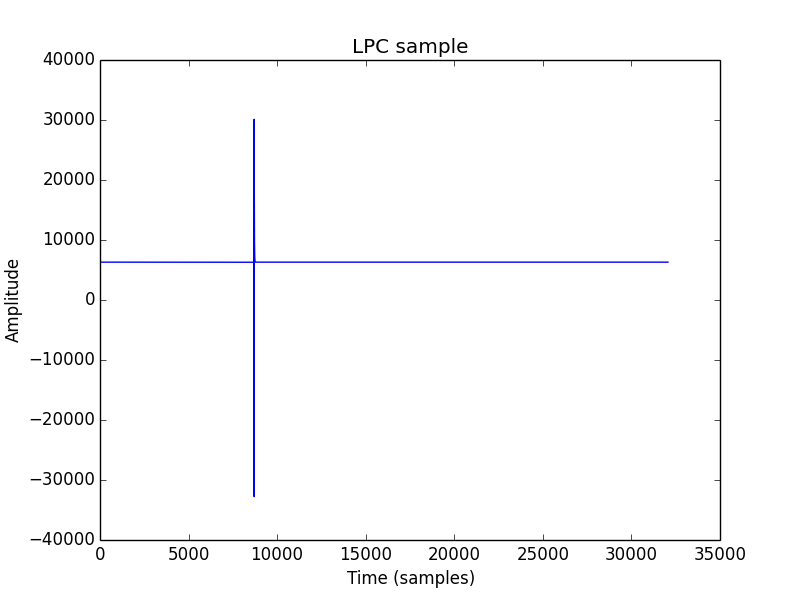
\includegraphics[width=0.6\textwidth,height=0.5\textwidth]{lpc_sample.png}
    \caption{Time domain sample from LPC model}
    \label{fig:lpc_sample}
\end{figure}

The neural network described in Table ~\ref{table:hyperparams} was trained a
small dataset of 50 speech samples, with some samples taken from the
TIMIT dataset and others taken from the LibriSpeech dataset. Training curves
for these two networks can be seen in Figures ~\ref{fig:sine_error} and
~\ref{fig:lpc_error}. These networks learned quite quickly, and reached
convergence within 100 epochs. Once training had converged, samples were
generated from each of the models. Some examples of these samples can be seen
in Figures ~\ref{fig:sine_sample} and ~\ref{fig:lpc_sample}.
\par
Both the LPC sample and the sine sample suffer from similar problems. In the
case of the LPC sample, the large instability around sample 7500 has completely
dominated the dynamic range of the signal, effectively zeroing out the original
signal. There are a number of reasons this
could be occurring. Since the output model
is Gaussian, it may accidentally draw very unlikely samples. Feeding this back
into the model may cause wild instabilities such as the ones seen in both
these cases. Alternatively, this could be an issue with LPC representations
specifically. Changing the LPC representation to LSF did not appear
to result in any noticeable stability improvements. It is likely that this 
problem could be partially removed by a smart postprocessing algorithm or
frame by frame gain normalization, but this is only treating the symptom of the
problem. Ultimately, there is something strange in the model itself or the 
representation which needs to be accounted for.
\par
Though the sine wave sample appears decent, and is audibly interesting, it is
still far from  far from true speech. The original signal is
distorted enough by the sinusoidal analysis process that
this generated sample is fairly indistinguishable from sinusoidal
versions of the original data. This is an
excellent result, and combined with conditional information or better training,
could lead to some interesting "robotic synthesizers" for text-to speech.
Though the sinusoid sample seems less unstable than the LPC sample, there are 
still some signs of instability around sample 12000. This leads credence to the
belief that this type of instability may be caused by poor or unlikely samples
from the mixture of Gaussians on the output of our network, which then feeds
back into the generation process. This could potentially move the RNN into
an unstable regime.

\section{Conclusion}
Speech processing is an interesting and broad research area, with a rich history
in signal processing and computer science literature. Using the TIMIT and
LibriSpeech datasets, we were able to train a recurrent neural network to
generate plausible speech-like data under a special representation.
Unfortunately, most of the samples generated were very poor, which may point
to issues in the representation, or issues with the conceptual model itself. 
More research will be needed to disentangle these two issues, but it is
reasonable to believe that solving these problems, along with adding the
ability to condition network generation, could lead to high quality samples and
an interesting system for speech synthesis.

\section*{Acknowledgments}
Special thanks to the LISA lab speech synthesis team. Much of the work here was
done in parallel with that project, and many small insights added up
to a lot of new knowledge over the course of the semester.

\section*{References}
\small{
[1] A. Graves, A. Mohamed, G. Hinton. "Speech Recognition with Deep Recurrent Neural Networks". ICASSP 2013, Vancouver, Canada. 
\par
[2] A. Graves. "Generating Sequences With Recurrent Neural Networks". arXiv:1308.0850.
\par
[3] V. Panayotov, G. Chen, D.Povey and S. Khudanpur,
"LibriSpeech: an ASR corpus based on public domain audio books". ICASSP 2015 (submitted)
\par
[4] J. Garofolo, L. Lamel, W. Fisher, J. Fiscus, D. Pallett, N. Dahlgren, V. Zue
"TIMIT Acoustic-Phonetic Continuous Speech Corpus LDC93S1". Linguistic Data Consortium, 1993.
\par
[5] B.S. Atal, M. Schroeder, "Predictive coding of speech signals and subjective error criteria," Acoustics, Speech, and Signal Processing, IEEE International Conference on ICASSP '78. , vol.3, no., pp.573,576, Apr 1978
\par
[6] X. Serra and J. O. Smith, "Spectral modeling synthesis: A sound analysis/synthesis system based on a deterministic plus stochastic decomposition," Computer Music Journal, vol. 14, no. 4, pp. 12-24, 1990.
\par
[7] A. Oppenheim, R.W. Schafer, J.R. Buck, J. R."Discrete-time signal processing. Upper Saddle River, N.J.: Prentice Hall.
\end{document}
